\documentclass[]{article}
 \usepackage{graphicx}
 \usepackage{multicol}
 \usepackage{graphicx}
 \usepackage{setspace}
 \singlespacing
%opening
\title{Analisi di un filtro crossover a tre vie passivo}
\author{Cristina Caprioglio, mat.0000975884, Luca Morelli , mat.0000976485}
\date{30 Maggio 2022}
\usepackage[margin=2cm]{geometry}
\usepackage{amsmath}

\begin{document}

\maketitle

\section{Abstract}
In questa esperienza abbiamo analizzato il comportamento di un filtro crossover a tre vie, in regime sinusoidale, composto da un filtro passa banda in parallelo con un passa basso e un passa alto. In particolare, abbiamo acquisito i dati relativi alla tensione e alle fasi in funzione della frequenza per ogni filtro, in modo da poter stimare i valori delle frequenze di crossover ($ \nu_{LM}=(487\pm19)\:Hz, \nu_{LH}=(684\pm44)\:Hz $ e $ \nu_{MH}=(1032\pm16)\:Hz $), che non sono risultati in accordo con quelli attesi ($ \nu_{LM}= (550 \pm 10) \:Hz, \nu_{LH}= (748
\pm 14 )\:Hz $ e $ \nu_{MH}= (1139\pm 21 )\:Hz $), e della frequenza di risonanza del filtro passa banda ($ \nu_{Ris}=(714\pm43)\: Hz$), che è invece risultato compatibile con quello teorico ($ \nu_{Ris}=(676\pm26)\: Hz$).
Studiando gli sfasamenti dei segnali filtrati rispetto alla sorgente abbiamo ottenuto un'ulteriore stima di $ \nu_{LH}=(700\pm16)\:Hz$ e di $ \nu_{0}=(737.4\pm6.0)\: Hz$ (frequenza caratteristica del filtro passa banda). Successive analisi ci hanno consentito di identificare come causa principale delle discrepanze la presenza di una resistenza interna al generatore che impedisce di erogare una tensione costante al variare della frequenza.

\section{Introduzione}
\hspace{\parindent}Il filtro crossover a tre vie passivo è un particolare tipo di circuito costituito da tre filtri (un passa basso, un passa banda ed un passa alto) posti in parallelo. Tale dispositivo permette di separare i segnali in entrata sui tre rami, ognuno destinato ad un particolare range di frequenze. Questo lo rende molto utile nella riproduzione musicale, in quanto permette di suddividere lo spettro sonoro da riprodurre in più porzioni, da destinare a più altoparlanti separatamente, ciascuno con la propria predisposizione meccanica. In particolare, il filtro passa basso, contenente un solo induttore e un solo resistore, destinato alla basse frequenze, è detto woofer, mentre il filtro passa alto, con un solo condensatore e un solo resistore,  selettivo per le frequenze superiori, è chiamato tweeter. Vi è quindi il ramo centrale, o di midrange, costituito da un RLC in serie che svolge il ruolo di filtro passa banda e si occupa delle frequenze intermedie. Il termine passivo deriva dal fatto che sono presenti solo componenti passivi, ovvero che non richiedono alimentazione esterna.\\
\hspace{\parindent}Il circuito è caratterizzato dalle frequenze di separazione dei vari filtri, che sono specifiche del circuito e sono dette \textit{frequenze di crossover}, ossia le frequenze alle quali due rami presentano la stessa tensione ai capi del proprio resistore. In particolare si dimostra (vedasi appendice) che le tre frequenze sono: 
\begin{equation}\label{crossoverLH}
 \nu_{LH}=\frac{1}{2\pi\sqrt{L_{L}C_{H}}}
\end{equation}
\begin{equation}\label{crossoverLM}
\nu_{LM}=\frac{1}{2\pi\sqrt{C_{M}(L_{M}+L_{L})}}
\end{equation}
\begin{equation}\label{crossoverMH}
	\nu_{MH}=\frac{1}{2\pi}\sqrt{\frac{2}{L_{M}C_{M}}}
\end{equation}
rispettivamente  $\nu_{LM}$ tra basso-medio,  $\nu_{LH}$ basso-alto e  $\nu_{MH}$ medio-alto. Inoltre è utile caratterizzare la frequenza di risonanza del ramo RLC data da:
\begin{equation}
  \nu_{Ris}=\nu_0 \sqrt{1-\frac{1}{2Q^2}} \quad  \nu_{0}=\frac{1}{2\pi\sqrt{L_M C_M}} \quad Q=\frac{1}{R_M}\sqrt{\frac{L_M}{C_M}}
\end{equation}
dove, per un fattore di qualità $(Q)$ molto elevato, $\nu_{Ris}$ tende a $\nu_{0}$. Si tenga conto che $\nu_{Ris}$ è la frequenza in cui la tensione misurata ai capi del resistore del midrange è massima mentre $\nu_{0}$ è la frequenza alla quale un'onda sinusoidale generata è in fase con quella misurata ai capi del resistore del ramo centrale, come mostrato nell'appendice. 
Inoltre $\nu_{0}$ dovrebbe avere un valore simile alla frequenza di crossover tra basso e alto.
Infine, come dimostrato nell'appendice, osserviamo che alla frequenza $\nu_{LH}$ la somma delle fasi del tweeter e del woofer è nulla.
\section{Apparato sperimentale e svolgimento}
\begin{figure}[h]
	\centering
	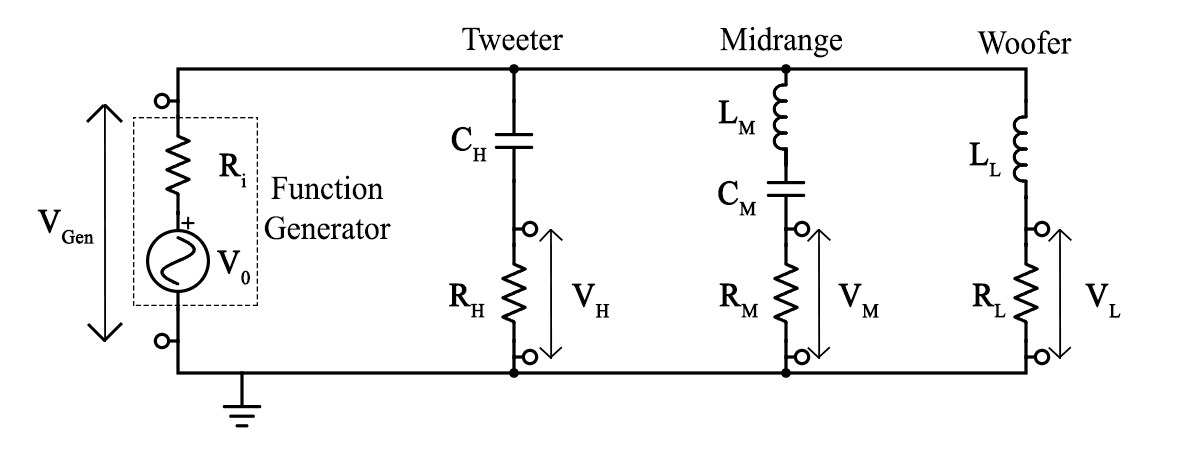
\includegraphics[width=1\linewidth]{img/Schema}
	Figura 1: \emph{Schema del circuito realizzato.}
\end{figure}

Il filtro crossover a tre vie, schematizzato in Fig. 1, che è stato da noi realizzato sulla breadboard della scheda di acquisizione dati NI ELVIS II, è composto da tre rami connessi in parallelo sottoposti ad una tensione variabile prodotta dal \textit{function generator} (a cui ci si riferirà anche come FGEN da qui in poi) di ELVIS.\\
\hspace*{\parindent}Il terzo ramo è il woofer ed é costituito da un induttore $ L_{L} = (45.2 \pm 1.2)\:mH $ ed una resistenza $ R_{L} = (155.02 \pm 0.17) \: \Omega $. Il secondo ramo é il midrange, con un induttore $ L_{M} = (39.5 \pm 1.1)\:mH $, un condensatore $ C_{M} = (0.9900 \pm 0.0099)\:\mu F $ ed una resistenza $ R_{M} = (153.20 \pm 0.17) \: \Omega $. Il primo ramo é infine il tweeter, su cui sono presenti un condensatore $ C_{H} = (1.00 \pm 0.01)\:\mu F $ ed una resistenza $ R_{H} = (149.96 \pm 0.17) \: \Omega $. Tutti i componenti dei singoli rami sono collegati in serie e condensatori ed induttori hanno resistenza interna che si è rivelata trascurabile rispetto alla resistenza di ogni resistore. Anche FGEN possiede una resistenza interna: $ R_{gen} = 50 \: \Omega $, dichiarata dal costruttore.\\
\hspace*{\parindent}I valori dei vari componenti sono stati misurati tramite il multimetro digitale di ELVIS e secondo il suo data sheet abbiamo calcolato gli errori strumentali. In particolare, per le induttanze abbiamo preso il valor medio su 4 misure poichè abbiamo constatato che in special modo il valore di queste è soggetto a fluttuazioni nell'arco di poche ore, che risultano maggiori dell'errore strumentale sulla misura, di conseguenza abbiamo considerato la semi dispersione massima delle 4 misure come errore.\\
\hspace*{\parindent}Per assicurarci del corretto funzionamento del circuito abbiamo prima di tutto analizzato l'andamento della tensione rispetto al tempo nei tre rami e nel generatore a 3 frequenze, rispettivamente una bassa, una media e una alta. Abbiamo quindi acquisito la tensione in ingresso $ V_{Gen} $ e quelle ai capi delle resistenze dei 3 rami al variare della frequenza. Per fare ciò abbiamo eseguito uno sweep tramite FGEN, facendo variare la frequenza tra $ 100 $ e $ 3000 \:Hz$ con step di $ 20 \:Hz $.\\ 
\hspace*{\parindent}Per l'acquisizione dei dati abbiamo usato un VI di LabView, da noi sviluppato, che facendo uso del subVI ``Extract Single Tone Information" ci ha permesso di estrarre per ogni acquisizione ampiezza, fase e frequenza del segnale di tensione. Occorre tener presente che lo sfasamento teorico atteso é rispetto a $ V_{Gen} $, pertanto dalla fase di ogni ramo abbiamo sottratto la fase misurata di FGEN. I dati sono stati acquisiti con una frequenza di campionamento di $ 100\: kHz $ e con numero di campioni pari a $ 2000 $ per acquisizione, in modo da avere un numero di punti per periodo sufficientemente elevato mantenendo la forma d'onda.\\
\hspace*{\parindent}Per ogni acquisizione effettuata abbiamo inoltre stimato l'errore sulla misura diretta acquisendo un semiperiodo di onda quadra, per la tensione in funzione del tempo, e un'onda di frequenza costante per le tensioni e fasi in funzione della frequenza. Utilizzando qualche centinaio di punti ciascuno abbiamo quindi calcolato la semi dispersione massima del campione che è stata utilizzata come stima dell'errore generato da FGEN e dall'apparato di acquisizione.\newpage
\section{Risultati e discussione}

\subsection{Analisi dell'andamento della tensione rispetto al tempo}
\hspace*{\parindent}In Fig.2 è possibile apprezzare le risposte dei filtri a tre frequenze distinte: come avevamo previsto, a basse frequenze l'ampiezza del woofer é la maggiore, nonché la più vicina a quella del generatore, mentre a medie frequenze é il midrange quello con il segnale più ampio. A $ 1500\: Hz$ invece vediamo che ad avvicinarsi all'ampiezza della sinusoide del generatore é il tweeter.\\
	\begin{multicols}{2}
		
		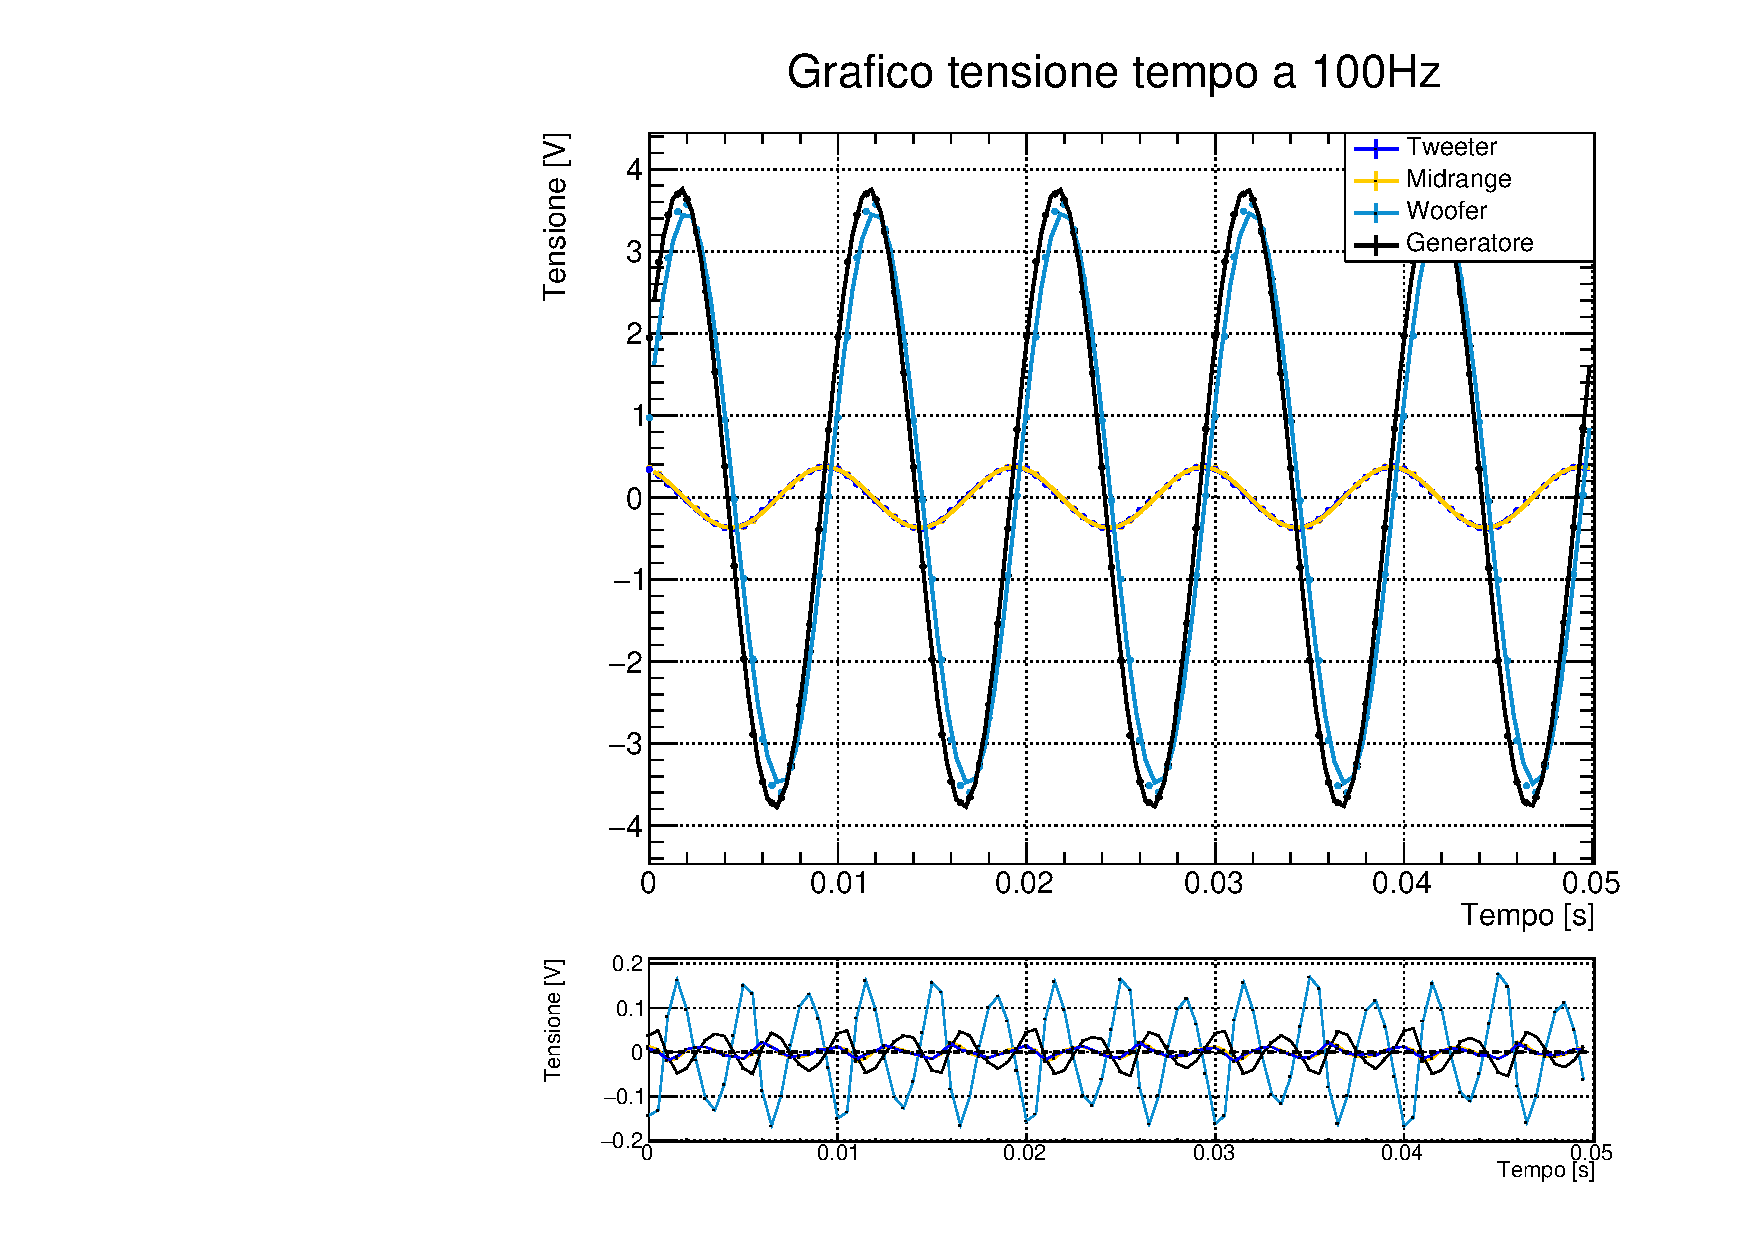
\includegraphics[width=1\linewidth]{img/100hz}
		
		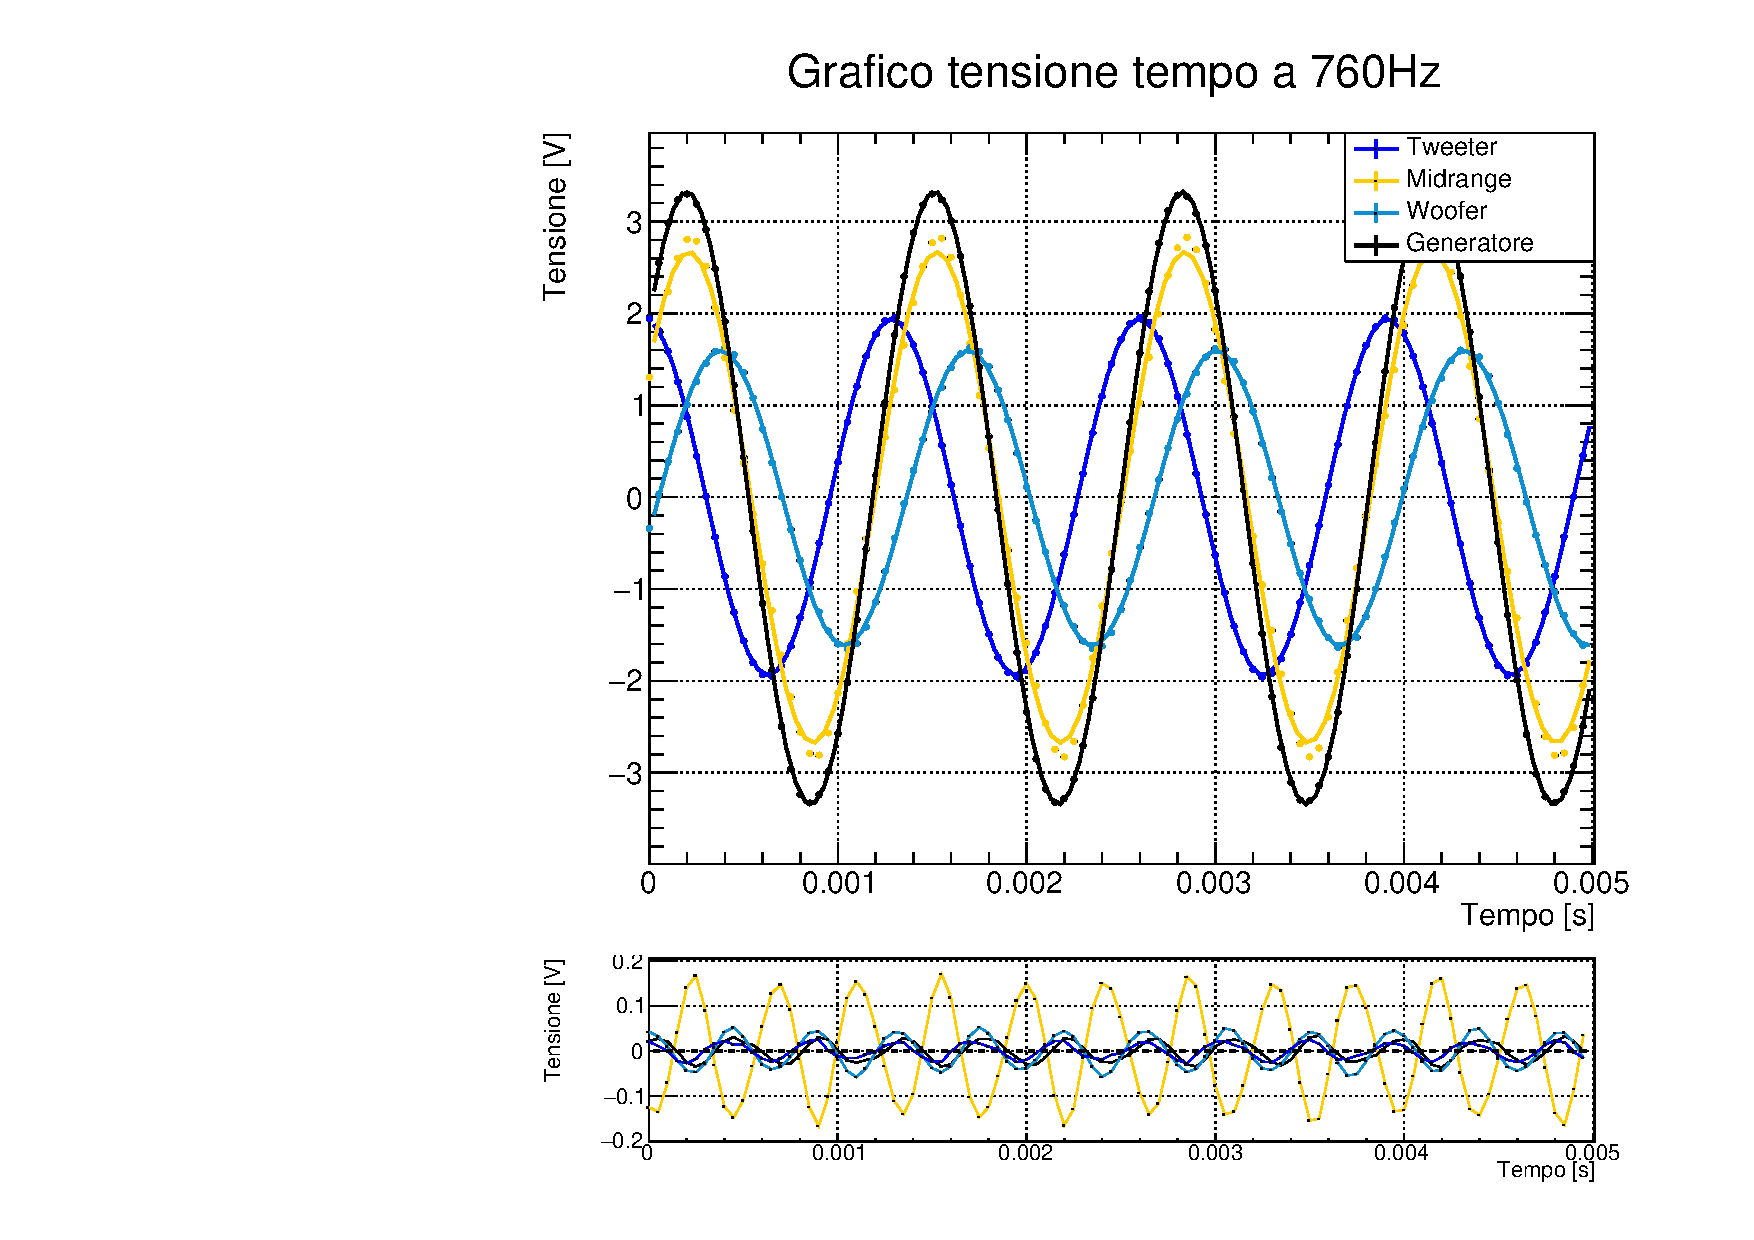
\includegraphics[width=1\linewidth]{img/760hz}
		
		
	\end{multicols}
	\makebox[\textwidth][c]{
		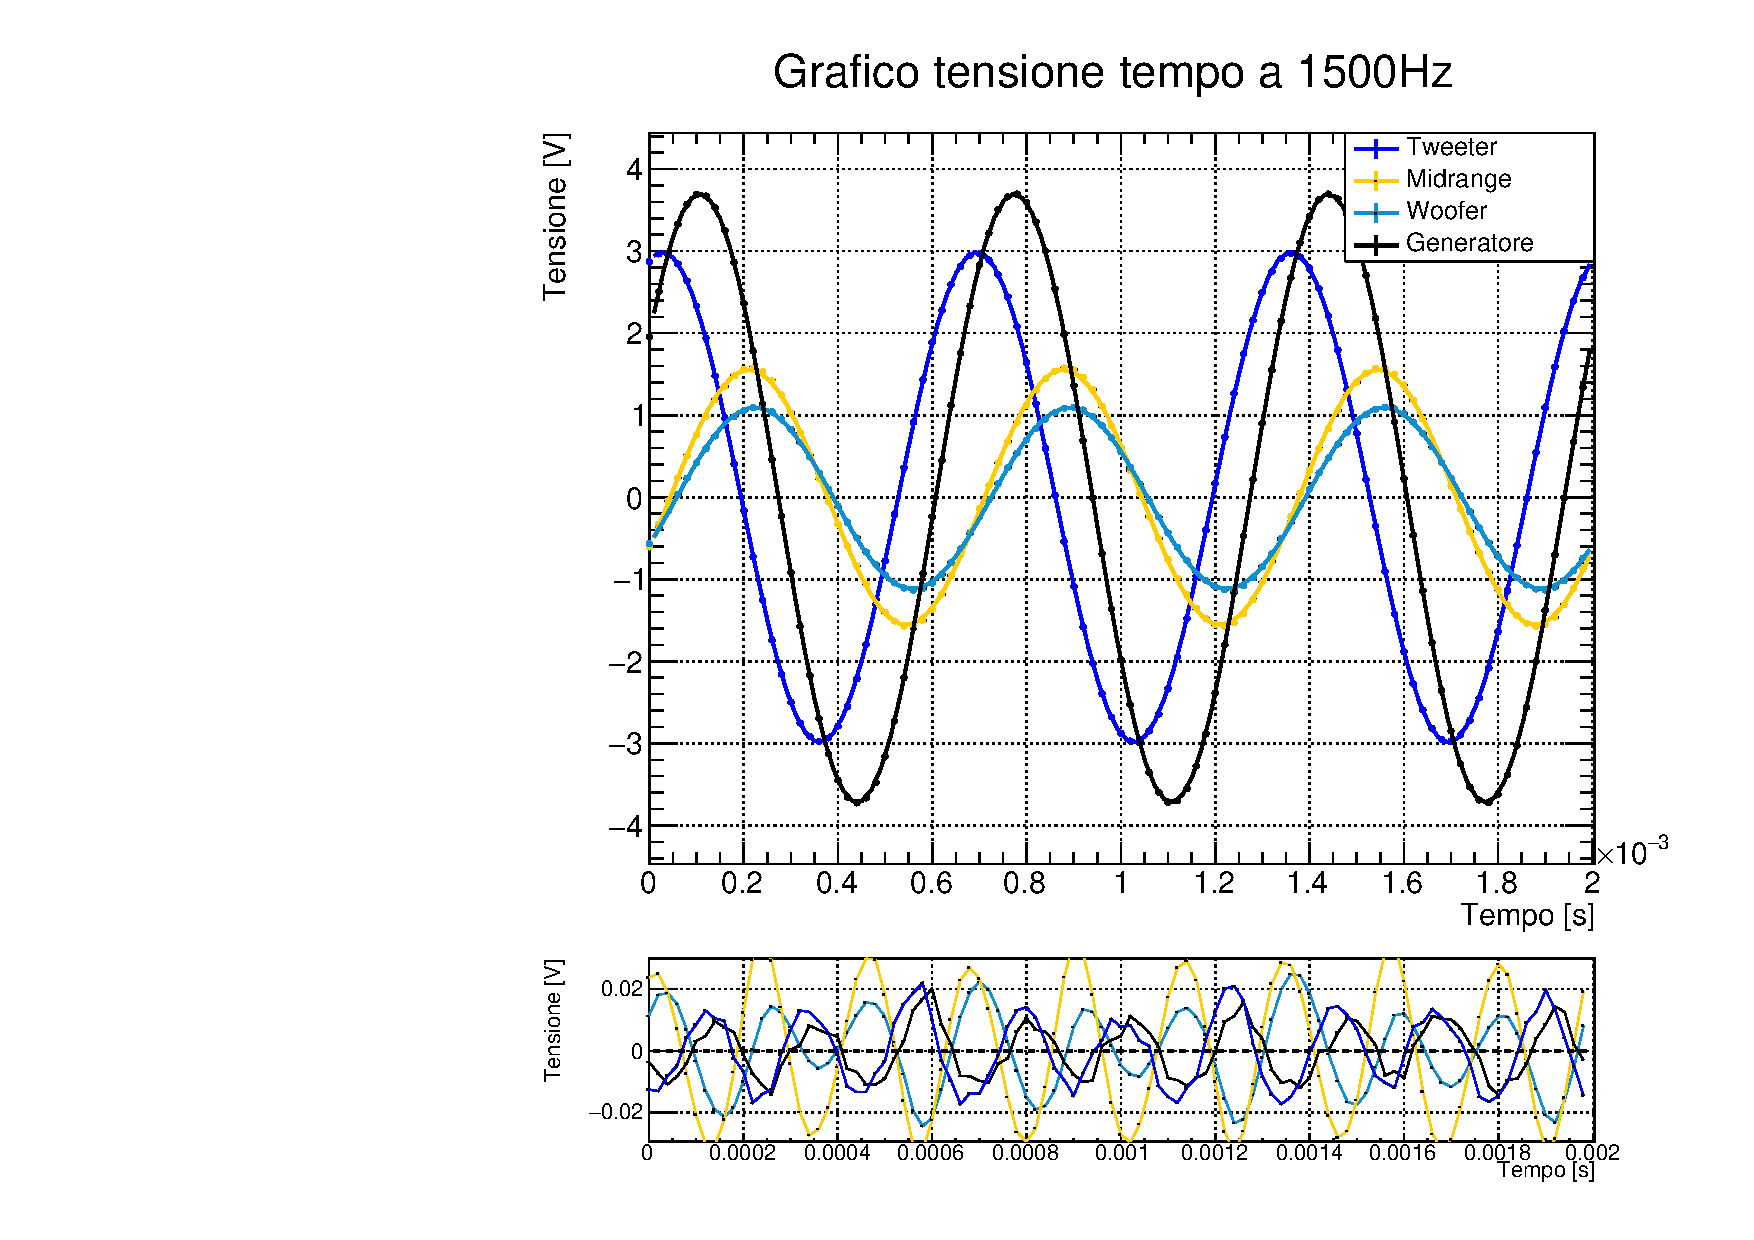
\includegraphics[width=0.5\linewidth]{img/1500hz}
	}

\begin{center}Figura 2: \emph{Risposta dei filtri in funzione del tempo a 100Hz, 760Hz e 1500Hz. Sono raffigurati sia i punti sperimentali acquisiti, le cui barre d'errore non sono visibili perchè troppo piccole per essere graficate, sia i risultati dei fit effettuati con un tratto continuo. Per ogni fit sono raffigurati gli scarti dai punti sperimentali in un apposito grafico sottostante che evidenzia la bontà del fit.}\\
	\end{center}

\newpage
Per ogni frequenza abbiamo effettuato fit con le funzioni che descrivono la tensione ai capi dei resistori dei singoli rami (riportate in appendice) che ci hanno permesso di confrontare, come riportato in Tab. 1, le ampiezze e le fasi misurate con quelle calcolate conoscendo le resistenze, le induttanze e le capacità del circuito.\\

\makebox[\textwidth][c]{
	\begin{tabular}{||l||c|c|c||}
		\hline
		Frequenza&Tweeter da fit&Midrange da fit&Woofer da fit \\ \hline \hline
		100Hz&$(0.3671\pm0.0014)V$&$(0.3719\pm0.0019)V$&$(3.486\pm0.016)V$\\
		760Hz&$(1.9371\pm0.0023)V$&$(2.671\pm0.015)V$&$(1.6036\pm0.0049)V$\\
		1500Hz&$(2.9870\pm0.0016)V$&$(1.6036\pm0.0031)V$&$(1.1036\pm0.0019)V$\\ \hline
  

\end{tabular}
}\\

\makebox[\textwidth][c]{
\begin{tabular}{||l||c|c|c||}
	\hline
	Frequenza&Tweeter atteso&Midrange atteso&Woofer atteso \\ \hline \hline
	100Hz&$(0.354\pm0.064)V$&$(0.356\pm0.064V$&$(3.707\pm0.030)V$\\
	760Hz&$(1.94\pm0.23)V$&$(3.30\pm0.39)V$&$(1.90\pm0.26)V$\\
	1500Hz&$(3.03\pm0.18)V$&$(1.83\pm0.29)V$&$(1.23\pm0.22)V$\\ \hline
	
	
\end{tabular} }\\

 \makebox[\textwidth][c]{
Tabella 1: \emph{Confronto delle ampiezze ottenute dai fit con quelle attese}}\\

Questa analisi preliminare evidenzia un buon grado di compatibilità tra le misure effettuate e i valori attesi, talvolta è però possibile notare una certa discrepanza, di cui discuteremo grazie ad ulteriori analisi che abbiamo condotto.
\subsection{Analisi della risposta in frequenza}


\hspace*{\parindent}In Fig.3 é rappresentato il grafico che permette di osservare l'andamento della tensione ai capi del resistore di ogni filtro e quella del generatore rispetto alla frequenza. Sempre in Fig.3 è presente il grafico che mostra gli sfasamenti dei segnali sui tre rami del circuito rispetto al segnale del generatore.
\begin{multicols}{2}
	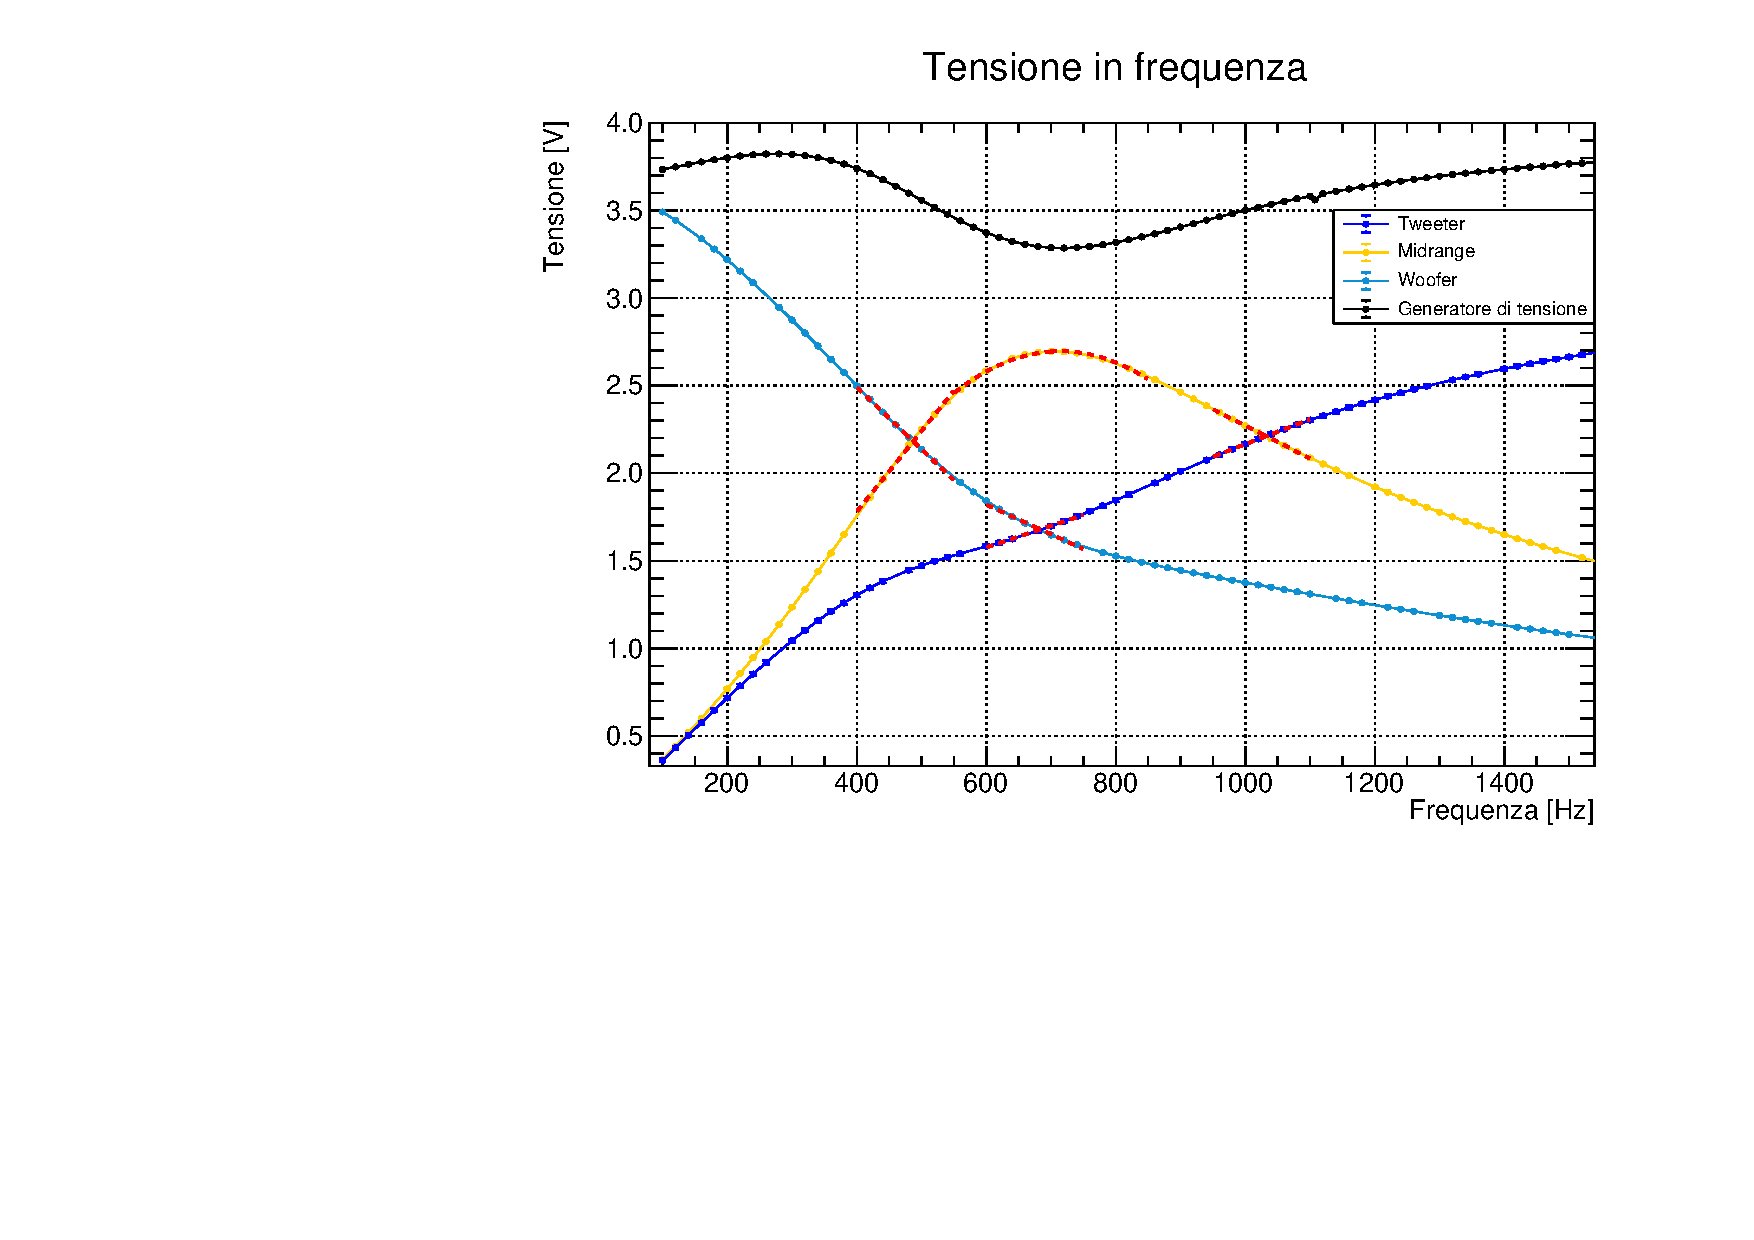
\includegraphics[width=1\linewidth]{img/Frequenza}	
	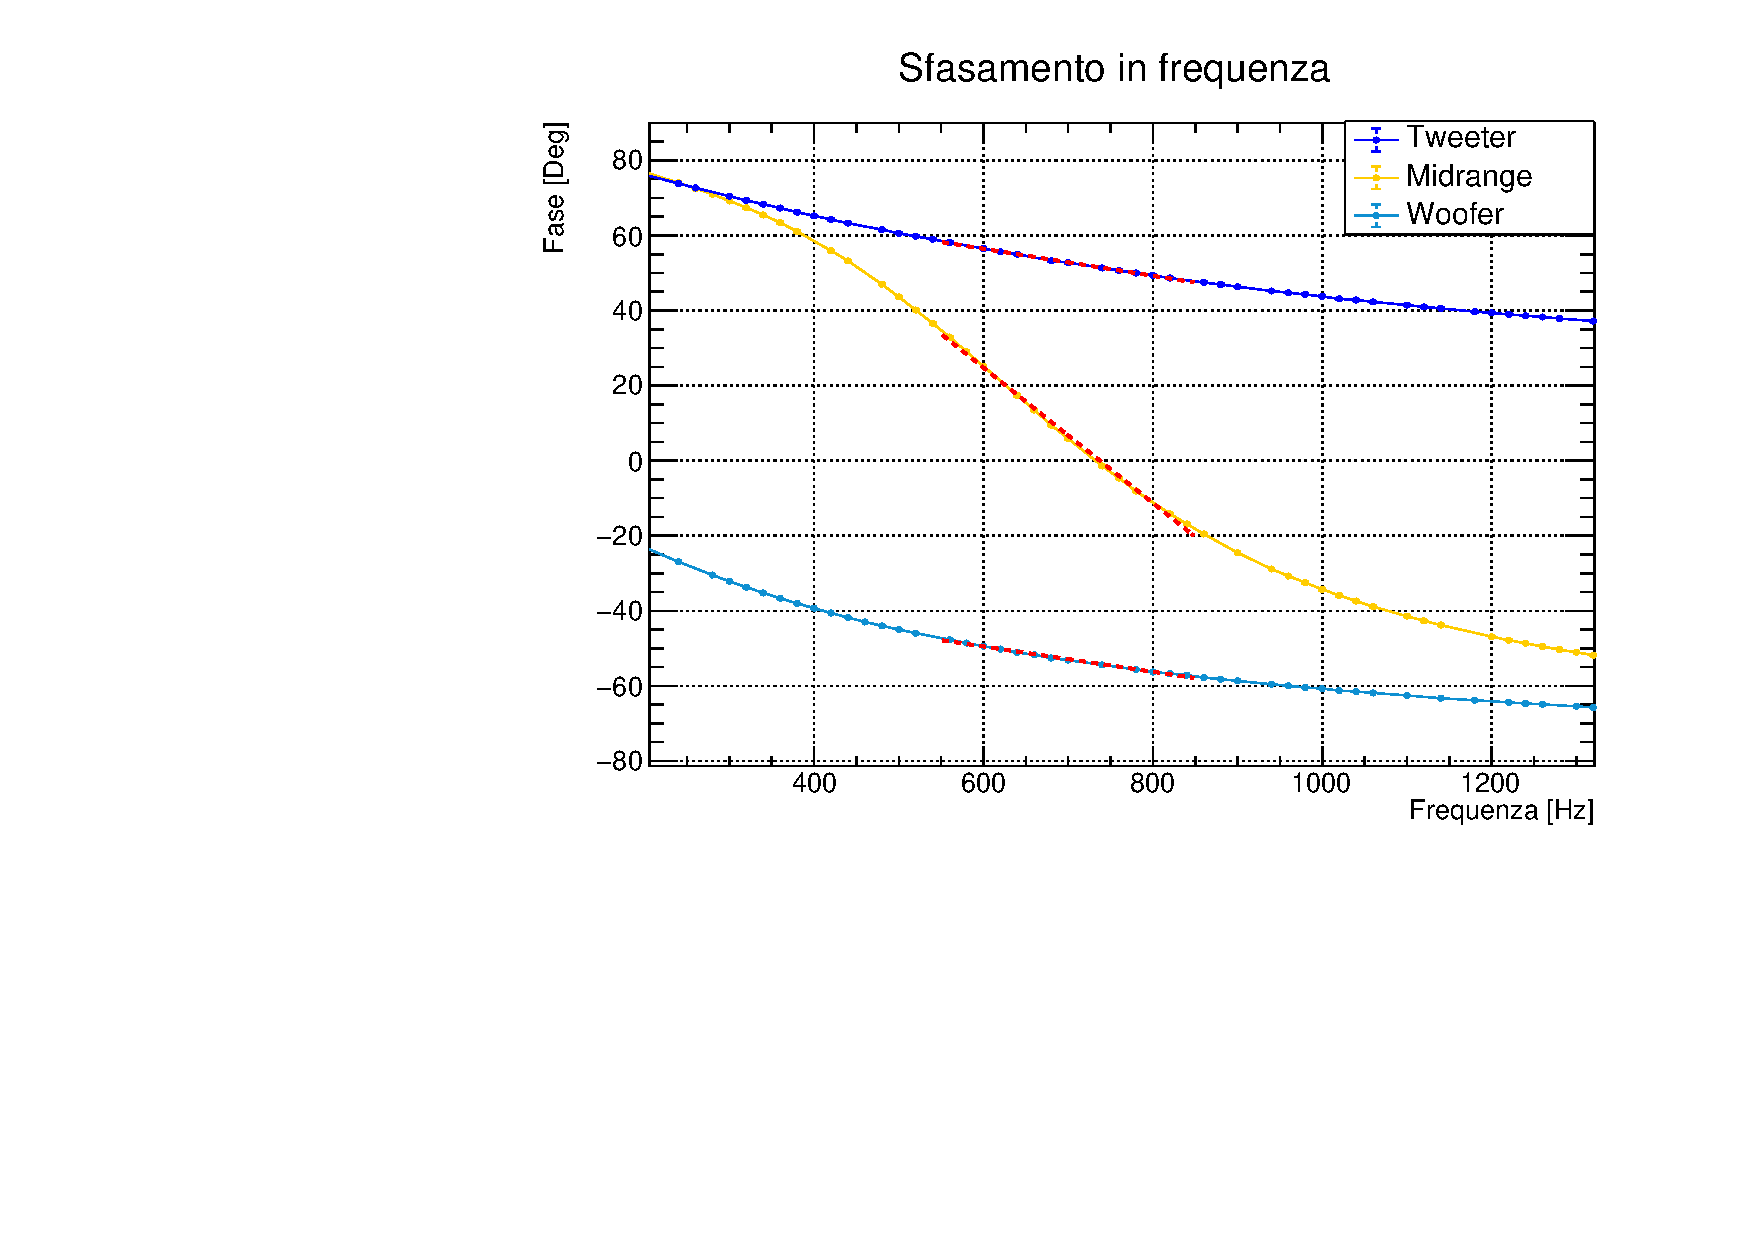
\includegraphics[width=1\linewidth]{img/Fasi}
\end{multicols}
\begin{center}
	Figura 3: \emph{Risposta in frequenza dei tre filtri. A sinistra è rappresentata l'ampiezza in funzione della frequenza mentre a destra gli sfasamenti rispetto al segnale del generatore. Sono raffigurati i punti sperimentali collegati da delle linee puramente grafiche, mentre sono state utilizzate delle linee rosse tratteggiate per i fit effettuati.}\\
\end{center}

Nel primo grafico è possibile apprezzare i punti in cui le tensioni di due rami si eguagliano, ossia i crossover, nonché il punto massimo della funzione relativa al circuito RLC. Per caratterizzare quantitativamente questi punti sono stati effettuati fit lineari nell'intorno dei crossover, così da poter ottenere il punto di intersezione, e fit a parabola nell'intorno del massimo, per ottenere quest'ultimo. Per quanto riguarda il ramo di midrange, dall'analisi dati si ottiene che il valore della frequenza di risonanza é pari a $ \nu_{Ris}=(714\pm43)\: Hz$, compatibile con il valore atteso $ \nu_{Ris}=(676\pm26)\: Hz$. Le frequenze di crossover rilevate ($ \nu_{LM}=(487\pm19)\:Hz,\: \nu_{LH}=(684\pm44)\:Hz\: $ e $\: \nu_{MH}=(1032\pm16)\:Hz $) non risultano in particolare accordo con i valori attesi ($ \nu_{LM}= (550 \pm 10) \:Hz,\: \nu_{LH}= (748
\pm 14 )\:Hz \:$ e $\: \nu_{MH}= (1139\pm 21 )\:Hz $). \\
\hspace*{\parindent}Per quanto concerne le fasi sono stati adoperati fit lineari nell'intorno dei punti interessati per poter identificare la frequenza in cui la fase del midrange si annulla, ossia in condizioni di prossimità a $\nu_0$, e quando la somma delle fasi del Tweeter e del Woofer si annulla, ossia nel punto di crossover dei due filtri. L'analisi dati ha restituito un valore della frequenza caratteristica del midrange di $ \nu_{0}=(737\pm23)\: Hz$ e di crossover tra tweeter e woofer pari a $ \nu_{LH}=(700\pm28)\:Hz$ che risultano in accordo entro gli errori stimati con i valori precedentemente misurati, ma non con quelli attesi ($ \nu_{0}=(805\pm15)\: Hz$).
\subsection{Analisi discrepanze}
\hspace*{\parindent}Una possibile causa delle discrepanze osservate tra risultati sperimentali e valori attesi è la presenza di una componente resistiva interna al Function Generator di ELVIS. Tutte le considerazioni teoriche fatte fino ad ora infatti si basano sull'assunzione che la resistenza interna del generatore si limiti ad aumentare la resistenza totale di ogni ramo senza variare la forma delle funzioni di trasferimento. Se questa assunzione non si rivelasse valida la resistenza del generatore dovrebbe causare una ulteriore caduta di potenziale in ogni ramo dipendente dalla frequenza di operazione.\\
\hspace*{\parindent}Come è possibile osservare in Fig. 3 questo è proprio quanto si verifica sperimentalmente, ossia che la tensione misurata ai capi del Function Generator ($V_{Gen}$ nello schema della Fig.1) non è costante, ma varia con la frequenza generata, modificando così i valori delle frequenze di crossover.
Per valutare quantitativamente quanto questo effetto influisca sulla misura abbiamo effettuato una serie di fit per ogni funzione di trasferimento in una regione del dominio delle frequenze in cui la tensione del generatore permane con buona approssimazione costante, similmente al comportamento supposto in origine.\\ 

\makebox[\textwidth][c]{
	\begin{tabular}{||c||r|r|r||}
		\hline
		Componenete&Tweeter&Midrange&Woofer \\ \hline \hline
		$R(\Omega)$&$(149.06\pm0.16)$&$(155.60\pm0.47)$&$(155.76\pm0.40)$\\
		$L(mH)$&&$(41.705\pm0.096)$&$(33.355\pm0.076)$\\
		$C(\mu F)$&$(0.7550\pm0.037)$&$(1.3633\pm0.00048)$&\\
		$\chi^2/NDF$&$1.34$&$1.61$&$1.57$\\\hline
		
		
\end{tabular} }
\begin{center}
	Tabella 3: \emph{Parametri restituiti dai fit delle funzioni di trasferimento di ogni ramo su un range ridotto tra i $1500Hz$ e i $3000Hz$. Per ogni ramo sono riportati i valori stimati delle sue componenti e il chi quadro ridotto del fit.}
\end{center}

In Tab.3 sono riportati i risultati dei fit effettuati tra i $1500Hz$ e i $3000Hz$, questi fit forniscono resistenze, capacità ed induttanze delle componenti di ogni ramo che sono quindi da confrontare con quelle misurate con il multimetro.  
Come è possibile osservare i dati ottenuti da questi fit evidenziano una maggiore aderenza dei punti sperimentali in questo range ridotto al modello teorico ipotizzato, evidenziando come una delle principali cause di errore, seppur non l'unica, sia da identificare negli effetti dovuti alla resistenza interna del function generator. \\
Inoltre, i valori più in accordo con le misure dirette sono quelli delle componenti resistive. Questa osservazione ci suggerisce che ulteriori fonti di errore siano da identificare nella misura delle induttanze e delle capacità: abbiamo infatti osservato che nell'arco di una mattinata il loro valore è risultato soggetto a fluttuazioni e per questo motivo si è considerato un valore medio tra più misure delle induttanze come miglior stima. Tuttavia, tale metodologia non si è rivelata sufficiente per tener conto di questo comportamento stocastico.  
\section{Conclusioni} 
L'esperimento ha parzialmente confermato il comportamento teorico del filtro che abbiamo studiato consentendo una stima dei valori delle frequenze di crossover $ \nu_{LM}=(487\pm19)\:Hz$,  $£ \nu_{LH}=(684\pm44)\:Hz $ e $ \nu_{MH}=(1032\pm16)\:Hz $ e di risonanza del circuito RLC  $ \nu_{Ris}=(714\pm43)\: Hz$. Se da un lato è risultata evidente la capacità filtrante del circuito, da un punto di vista quantitativo le frequenze caratteristiche del circuito misurate non si sono rivelate in pieno accordo con quelle attese. Ulteriori analisi ci hanno permesso di identificare come sorgente principale di tali errori la presenza di una resistenza interna del generatore di tensione, che influisce sulle funzioni di trasferimento dei singoli rami. Tale effetto è facilmente osservabile studiando la tensione generata a frequenze diverse, la quale non si è rivelata essere costante come supposto. Abbiamo inoltre osservato che un'ulteriore fonte di errore non trascurabile è dovuta alle fluttuazioni dei valori delle componenti non resistive che si manifestano nell'arco di poche ore dalla misura.
\newpage
{\large\textbf{Appendice: }}
Tutte le formule sono state ricavate tramite il formalismo dei fasori. Per ricavare le formule è stata considerata la resistenza di FGEN $ R_{gen} $, considerando però i singoli rami indipendenti tra loro.\\
Utilizzando la legge per le maglie di Kirchhoff su ogni ramo del circuito abbiamo ricavato la funzione di trasferimento di ogni filtro, il cui modulo regola la tensione misurata sul ramo e il cui argomento regola la fase.\\
$ \bullet \: $\textbf{Formule per il woofer} {\small\emph{($V_L=R_L I$)}}
\begin{equation}\label{V_{L}}
	\vec{V_0}=(R_{gen}+R_L+ \frac{1}{j\omega C_L})\vec{I}\quad  \Longrightarrow \quad \lvert H(\omega)\rvert=\frac{	\lvert \vec{ V_{L}} \rvert}{\lvert \vec{ V_{0}} \rvert}=\frac{1}{\sqrt{\frac{(R_{gen}+R_{L})^2}{R_{L}^{2}}+\frac{\omega^{2}L_{L}^{2}}{R_{L}^{2}}}}
\end{equation}
$ \bullet \: $\textbf{Formule per il tweeter} {\small\emph{($V_H=R_H I$)}}
\begin{equation}\label{V_{H}}
\vec{V_0}=(R_{gen}+R_H+j\omega L_H)\vec{I} \quad \Longrightarrow \quad \lvert H(\omega)\rvert=\frac{	\lvert \vec{V_H} \rvert}{\lvert \vec{V_0}\rvert} =\frac{1}{\sqrt{\frac{(R_{gen}+R_{H})^{2}}{R_{H}^{2}}+\frac{1}{\omega^{2}C_{H}^{2}R_{H}^{2}}}}
\end{equation}
$ \bullet \: $\textbf{Formule per il midrange} {\small\emph{($V_M=R_M I$)}}
\begin{equation}\label{V_{M}}
	\vec{V_0}=(R_{gen}+R_M+ \frac{1}{j\omega C_M}+j\omega L_M)\vec{I} \quad \Longrightarrow \quad \lvert H(\omega)\rvert=\frac{	\lvert \vec{V_M} \rvert}{\lvert \vec{V_0} \rvert}=\frac{1}{\sqrt{\frac{(R_{gen}+R_{L})^{2}}{R_{M}^{2}}+\frac{1}{R_{M}^{2}}\left( \omega L_{M}-\frac{1}{\omega C_{M}}\right) ^{2}}}
\end{equation}
\textbf{Formule per le frequenze di crossover}\\
Per trovare le frequenze di crossover abbiamo eguagliato i moduli delle funzioni di trasferimento dei rami due a due e ricavato $\omega$. In tutte e tre le formule, nonostante il loro valore non fosse identico, sono state semplificate le resistenze poichè l'errore dovuto a questa approssimazione si è rivelato inferiore a quello sulla misura. Per analoghe motivazioni abbiamo considerato le capacità con lo stesso valore (Eq.(10)). Non è invece stato possibile effettuare la stessa approssimazione anche per le induttanze (Eq.(9)).\\
$ \bullet  \:$\textbf{Crossover tra woofer e tweeter:}
L'Eq.(1) si ottiene da:
\begin{equation}\label{crossoverLH_H}
	\frac{1}{\sqrt{\frac{(R_{gen}+R_{L})^{2}}{R_{L}^{2}}+\frac{\omega^{2}L_{L}^{2}}{R_{L}^{2}}}}=\frac{1}{\sqrt{\frac{(R_{gen}+R_{H})^{2}}{R_{H}^{2}}+\frac{1}{\omega^{2}C_{H}^{2}R_{H}^{2}}}} \quad \Longrightarrow \quad \nu_{LH}=\frac{\omega_{LH}}{2\pi}=\frac{1}{2\pi\sqrt{L_{L}C_{H}}}
\end{equation}
$ \bullet \: $\textbf{Crossover tra woofer e midrange:}
L'Eq.(2) si ottiene da:
\begin{equation}\label{crossoverLM_H}
\frac{1}{\sqrt{\frac{(R_{gen}+R_{L})^{2}}{R_{L}^{2}}+\frac{\omega^{2}L_{L}^{2}}{R_{L}^{2}}}}=\frac{1}{\sqrt{\frac{(R_{gen}+R_{M})S^{2}}{R_{M}^{2}}+\frac{1}{R_{M}^{2}}\left( \omega L_{M}-\frac{1}{\omega C_{M}}\right) ^{2}}} \quad  \Longrightarrow \quad \nu_{LM}=\frac{\omega_{LM}}{2\pi}=\frac{1}{2\pi\sqrt{C_{M}(L_{M}+L_{L})}}
\end{equation}
$ \bullet  \:$\textbf{Crossover tra midrange e tweeter:} 
L'Eq.(3) si ottiene da:
\begin{equation}\label{crossoverMH_H}
	\frac{1}{\sqrt{\frac{(R_{gen}+R_{M})^{2}}{R_{M}^{2}}+\frac{1}{R_{M}^{2}}\left( \omega L_{M}-\frac{1}{\omega C_{M}}\right) ^{2}}}=\frac{1}{\sqrt{\frac{(R_{gen}+R_{H})^{2}}{R_{H}^{2}}+\frac{1}{\omega^{2}C_{H}^{2}R_{H}^{2}}}} \quad \Longrightarrow \quad \nu_{MH}=\frac{\omega_{MH}}{2\pi}=\frac{1}{2\pi}\sqrt{\frac{2}{L_{M}C_{M}}}
\end{equation}
%Se si sviluppasse esattamente i calcoli si vedrebbe che invece di $ \sqrt{2} $ a numeratore dovrebbe comparire \\
%$ \sqrt{1+\sqrt{1-1.96\times 10^{-28}}} $, che é però approssimabile a $ \sqrt{2} $.\\
\textbf{Considerazioni sulle fasi}\\
Alla frequenza di crossover tra tweeter e woofer $\nu_{LH}$ (vedi Eq.(1)), considerando $ R_{L} \approx R_{H} $, si avrà:
\begin{equation}
\phi_{L}(\nu_{LH})+\phi_{H}(\nu_{LH})  = \arctan \left( -\frac{2\pi\frac{1}{2\pi\sqrt{L_{L}C_{H}}} L_{L}}{(R_{gen}+R_{L})}\right)+\arctan \left( \frac{1}{2\pi\frac{1}{2\pi\sqrt{L_{L}C_{H}}} (R_{gen}+R_{H})C_{H}}\right)=0 
\end{equation} 
Alla frequenza caratteristica del ramo midrange $\nu_{0}$ (vedi Eq.(4)) si avrà:
\begin{equation}
	\phi_{M}(\nu_{0})=\arctan \left( \frac{1-(2\pi\frac{1}{2\pi\sqrt{L_M C_M}})^{2}L_{M}C_{M}}{ 2\pi\frac{1}{2\pi\sqrt{L_M C_M}} (R_{gen}+R_{L})C_{M}}\right)=\arctan \left( \frac{0}{ 2\pi\frac{1}{2\pi\sqrt{L_M C_M}} (R_{gen}+R_{L})C_{M}}\right)=0
\end{equation}
\end{document}
